\documentclass[11pt,a4paper]{article}
\usepackage[T1]{fontenc}
\usepackage[utf8]{inputenc}
\usepackage[margin=2.5cm]{geometry}
\usepackage{amsmath,amssymb}
\usepackage{booktabs,array,longtable,graphicx,xcolor,setspace,caption}
\usepackage[authoryear,round]{natbib}
\usepackage[colorlinks=true,linkcolor=blue!50!black,citecolor=blue!50!black,urlcolor=blue!50!black]{hyperref}
\setstretch{1.15}
\newif\ifdraft \drafttrue
\newcommand{\todo}[1]{\ifdraft{\color{red}\textbf{[TODO: #1]}}\fi}
\newcommand{\PS}{\mathit{PS}}
\newcommand{\RepoDOI}{10.5281/zenodo.XXXXXXX}   % <- paste the DOI of the corrected Zenodo release here

\title{Tourism Yield and Spatial Concentration in Thailand:\\ A Provincial Assessment Using the Punch Score}
\date{}
\begin{document}
\maketitle

\begin{abstract}
\noindent This study examines provincial tourism yield and spatial concentration across all 77 provinces of Thailand in 2024. It applies the Punch Score, a relative-yield index comparing each province's share of national tourism receipts with its share of recorded visits. Bangkok and the South account for 33.2\% of visits and 65.9\% of receipts. Seven provinces exceed the national yield benchmark. The provincial Gini coefficients are 0.827 for receipts and 0.558 for visits, while between-region differences account for approximately 60.0\% of Theil inequality in receipts. Foreign visitors represent 23.5\% of recorded visits and 61.5\% of receipts. Visitor composition accounts for approximately 44.6\% of the cross-provincial variance in receipts per visit. Positive spatial autocorrelation is observed, with high-yield clustering along the southern coast. The study is descriptive and uses nominal gross receipts; it does not establish causal effects or measure tourism-sector productivity.

\medskip\noindent\textbf{Keywords:} tourism yield; regional inequality; location quotient; Theil decomposition; spatial autocorrelation; Thailand
\end{abstract}

\section{Introduction}
Tourism policy is frequently evaluated through visitor arrivals. Although arrivals measure the volume of destination activity, they do not indicate how much economic revenue those visits generate. Destinations with similar visit counts can record substantially different receipts because of differences in visitor composition, length of stay, accommodation use, and expenditure patterns \citep{wang2010,brida2013}. In a country such as Thailand, where tourism activity is distributed across a metropolitan centre, internationally marketed coastal destinations, and provinces serving predominantly domestic travellers, visitor counts alone may therefore provide an incomplete account of the geographical distribution of tourism receipts.

This study documents the relationship between recorded visits and tourism receipts across all 77 Thai provinces in 2024. It applies the Punch Score, which divides a province's share of national tourism receipts by its share of national recorded visits and scales the result so that 100 represents the national average. The index is a relative-yield measure with a structure analogous to a location quotient in regional analysis \citep{isard1960}. It is algebraically equivalent to a rescaling of receipts per recorded visit. The term Punch Score is retained for continuity with related methodological work on a weighted multi-criteria Punch Score framework \citep{anon2026b,anon2026}; the index used here is the single-criterion, risk-neutral special case defined in Section~\ref{sec:ps}, and it is not presented as a new theoretical construct.

The contribution of this paper is empirical rather than methodological. It combines a provincial relative-yield measure with analyses of the geographical concentration of receipts and visits, the decomposition of inequality across regions, visitor composition, and spatial autocorrelation. The analysis addresses four questions:
\begin{enumerate}
\item How unevenly are tourism receipts and recorded visits distributed across Thailand's provinces?
\item How much of the geographical variation in receipts per visit is associated with differences in the shares of Thai and foreign visitors, and how much is associated with within-type receipts per visit?
\item Do provincial tourism yields exhibit global and local spatial clustering?
\item Are the principal descriptive findings sensitive to excluding Bangkok?
\end{enumerate}
The analysis is descriptive. It uses one calendar year, nominal gross receipts, and aggregate recorded visits. It does not identify causal determinants of provincial yield, estimate tourism-sector productivity, or measure the proportion of tourism receipts retained as local value added.

\section{Background and conceptual framework}
\subsection{Tourist expenditure and relative yield}
Aggregate tourism receipts can be expressed as the product of recorded visits and average receipts per visit. Consequently, a province's share of national receipts reflects both its share of visits and its relative yield. Tourist expenditure varies across individuals, trip purposes, destination characteristics, and travel contexts \citep{wang2010,brida2013}. Visitor arrivals therefore cannot be treated as a direct proxy for the economic receipts generated by tourism.

Destination competitiveness frameworks identify resources, supporting factors, destination management, and demand conditions as relevant to tourism outcomes \citep{dwyer2003}. A yield index can be interpreted as an outcome indicator within this broader framework, but it does not measure destination competitiveness itself. In particular, high receipts per visit do not necessarily indicate higher productivity, better management, or greater local economic welfare.

\subsection{Relative-share indices and spatial concentration}
Location quotients compare a unit's share of an activity with its share of a reference total. Revealed comparative advantage uses a related relative-share logic to compare export structures \citep{isard1960,balassa1965}. The Punch Score applies this general approach to tourism receipts relative to recorded visits. It identifies provinces whose receipts per visit are above or below the national average.

New Economic Geography emphasises the role of market access, transport costs, and increasing returns in the geographical concentration of economic activity \citep{krugman1991}. In tourism, established destination brands, accommodation capacity, transport connectivity, and international market access may reinforce the position of leading destinations. These mechanisms provide possible interpretations of geographical concentration, but they cannot be tested directly with the single-year descriptive data used here.

Regional inequality has long been examined as part of the process of national development \citep{williamson1965}. Tourism has also been studied in relation to income inequality and economic growth \citep{alam2016,balaguer2002,brida2016}. However, gross tourism receipts are not equivalent to regional value added, household income, or local welfare. The geographical distribution of receipts should therefore be interpreted as a measure of where gross tourism spending is recorded rather than where all resulting economic benefits accrue.

\subsection{Measurement of inequality and spatial association}
The Gini coefficient and Lorenz curve provide summaries of distributional concentration \citep{cowell2011}. Theil's entropy measure is particularly useful because it can be decomposed into between-group and within-group components \citep{theil1967,shorrocks1980}. This allows the analysis to distinguish inequality associated with differences among regions from inequality among provinces within the same region.

Spatial autocorrelation measures the extent to which values observed at geographically related locations are similar. Global Moran's $I$ provides a summary measure of spatial association \citep{moran1950}, while local indicators of spatial association identify local clusters and spatial outliers \citep{anselin1995}. These methods are applied to provincial tourism yield to examine whether high- and low-yield provinces are spatially clustered.

\section{Data and methods}
\subsection{Data sources and geographical coverage}
The analysis covers all 77 provinces of Thailand for calendar year 2024 (B.E.\ 2567). Provincial visits, receipts, Thai and foreign visitor components, accommodation guests, and occupancy rates are taken from the revised provincial tourism-statistics workbook issued by the Ministry of Tourism and Sports and identified in the workbook as revised on 28 August 2025 \citep{mots2025a}.

Accommodation rooms, length of stay, and average daily expenditure are taken from the Ministry's Domestic Tourism Statistics workbooks for 2024. Gross provincial product (GPP) at current prices is taken from the National Economic and Social Development Council \citep{nesdc2025}. Registered population and provincial area are taken from National Statistical Office publications \citep{nso2025,nso2026}. Province centroids are calculated from the provincial administrative-boundary dataset distributed through the United Nations Office for the Coordination of Humanitarian Affairs' Humanitarian Data Exchange \citep{ocha2019}.

Bangkok is treated as a separate geographical category. The remaining 76 provinces are grouped into five regions: Central (including the West), East, North, Northeast, and South. The corresponding province counts are 17, 8, 17, 20, and 14, respectively.

Recorded visits are not counts of unique individual travellers. A traveller visiting more than one province may be recorded in each province visited. Provincial visit totals therefore represent recorded destination visits and should not be interpreted as the number of distinct national trips.

Tourism receipts are official gross-receipt estimates. They are nominal, are not adjusted for provincial price-level differences, and are not measures of value added. Length of stay and expenditure variables originate from the same tourism-statistics system as the receipts estimates. Their associations with receipts per visit may therefore be partly definitional rather than independent evidence of explanatory relationships.

\subsection{Data validation}
The assembled provincial dataset was checked for the following conditions before analysis: (1) exactly 77 unique provincial observations; (2) Thai and foreign visits sum to total visits within each province; (3) Thai and foreign receipts sum to total receipts within each province; (4) provincial visits, receipts, accommodation guests, and rooms reconcile with the corresponding published regional and national totals; and (5) no provincial value is replaced or imputed. The checks are reproduced by the dataset-construction script in the supplementary material.

The sum of provincial GPP is THB 18,683,881 million, compared with the published national total of THB 18,683,885 million. The difference of THB 4 million is treated as a source-level rounding discrepancy and is not adjusted.

\subsection{Punch Score}\label{sec:ps}
Let $R_i$ and $V_i$ denote tourism receipts and recorded visits in province $i$, respectively. National totals are $R=\sum_{i=1}^n R_i$ and $V=\sum_{i=1}^n V_i$. Provincial receipts per recorded visit are $y_i=R_i/V_i$, while the national benchmark is $\bar y=R/V$. The Punch Score is defined as a quantitative relative-yield scoring measure:
\begin{equation}
\PS_i=100\times\frac{R_i/R}{V_i/V}=100\times\frac{y_i}{\bar y}.
\end{equation}
It is a dimensionless index normalized to the national benchmark of 100, not a percentage. A score of 150, for example, indicates that receipts per recorded visit are 1.5 times the national average, or 50\% above the benchmark. A score above 100 indicates receipts per recorded visit above the national average, whereas a score below 100 indicates a yield below the national average. The identity
\begin{equation}
\frac{R_i}{R}=\frac{V_i}{V}\times\frac{\PS_i}{100}
\end{equation}
shows that a province's share of national receipts is the product of its share of recorded visits and its relative yield. The index is therefore a transparent descriptive measure of relative receipts per visit, not a measure of technical efficiency or productivity.

\paragraph{Relation to the Punch Score framework.} In related methodological work the Punch Score is defined as a composite scoring structure, $S_i=Z_iw/(1+\lambda r_i)$: a weighted aggregation of standardised benefit criteria $Z_i$ with a weight vector $w$ ($w_j\ge0$, $\sum_j w_j=1$), divided by a separately specified multiplicative risk adjustment with risk measure $r_i\ge0$ and penalty parameter $\lambda\ge0$ (written $R_i$ there and renamed here because $R_i$ denotes receipts) \citep{anon2026b,anon2026}. That work does not require identical criteria, normalisation procedures or risk variables in every application. The provincial index in Equation~(1) is the special case with a single benefit criterion (receipts per recorded visit, standardised by division by its national value, $Z_i=y_i/\bar y$), unit weight, and no risk adjustment ($\lambda=0$), multiplied by 100 for presentation: $\PS_i=100\,S_i$. It is therefore not the multi-criteria framework itself. It involves no weights, no risk term, and no estimation of weights from outcomes, and nothing in this paper evaluates that framework. Because the index has a single criterion, rankings do not depend on the form of standardisation.

\subsection{Concentration measures}
For a non-negative provincial variable $x_i$, let $x_{(1)}\le\cdots\le x_{(n)}$ denote the observations ordered from smallest to largest. The unweighted Gini coefficient is calculated as
\begin{equation}
G=\frac{2\sum_{i=1}^n i\,x_{(i)}}{n\sum_{i=1}^n x_i}-\frac{n+1}{n}.
\end{equation}
Lorenz curves plot cumulative shares of the variable against cumulative shares of provinces. Theil's $T$ is calculated as
\begin{equation}
T=\sum_{i=1}^n s_i\ln(ns_i),\qquad s_i=\frac{x_i}{\sum_{j=1}^n x_j}.
\end{equation}
For regions $g$ containing $n_g$ provinces and accounting for share $S_g$ of the national total, Theil's $T$ is decomposed into between-region and within-region components:
\begin{align}
T&=T_{\text{between}}+T_{\text{within}},\\
T_{\text{between}}&=\sum_g S_g\ln\!\Big(\frac{S_g}{n_g/n}\Big),\\
T_{\text{within}}&=\sum_g S_g T_g.
\end{align}
Provinces are equally weighted units in the baseline Gini and Theil calculations. The resulting statistics describe inequality across provinces, not inequality among tourists, households, or residents.

The reported bootstrap intervals are based on 10,000 resampling replications in which provinces are resampled within their respective regions; they are 2.5th and 97.5th percentiles. Because the dataset covers the complete set of 77 provinces rather than a random sample of provinces, these intervals are interpreted as conditional resampling intervals that describe sensitivity to the provincial distribution under the specified resampling scheme. They are not conventional design-based confidence intervals for a sample drawn from a larger population of Thai provinces.

A population-weighted sensitivity analysis is also reported for receipts per resident. Its interpretation differs from the baseline equal-province analysis because larger populations receive greater weight.

\subsection{Visitor-composition decomposition}
Let $f_i$ denote the foreign share of recorded visits in province $i$, and let $f$ denote the corresponding national share. Let $y_{T,i}$ and $y_{F,i}$ denote receipts per Thai and foreign recorded visit in province $i$. The national receipts-per-visit benchmarks for Thai and foreign visitors are denoted by $\bar y_T$ and $\bar y_F$.

Because total receipts are additive across visitor types, provincial receipts per visit can be decomposed as
\begin{equation}
y_i-\bar y=\underbrace{(f_i-f)(\bar y_F-\bar y_T)}_{\text{composition effect}}+\underbrace{(1-f_i)(y_{T,i}-\bar y_T)+f_i(y_{F,i}-\bar y_F)}_{\text{within-type rate effect}}.
\end{equation}
The composition term captures the difference associated with a province's foreign-visitor share relative to the national share, holding national visitor-type yields fixed. The within-type term captures differences between provincial and national receipts per visit within each visitor type.

The contribution of each component to cross-provincial variance is calculated as its covariance with total receipts per visit divided by the variance of total receipts per visit:
\begin{equation}
C_k=\frac{\operatorname{Cov}(y_i,d_{k,i})}{\operatorname{Var}(y_i)},
\end{equation}
where $d_{k,i}$ denotes the relevant decomposition component. The two covariance shares sum to one when the decomposition identity is satisfied and all terms are calculated using the same provincial observations and weighting convention. These shares are descriptive accounting decompositions, not causal effects.

\subsection{Spatial analysis}
Global spatial autocorrelation is assessed using Moran's statistic:
\begin{equation}
I=\frac{n}{W}\,\frac{\sum_i\sum_j w_{ij}(x_i-\bar x)(x_j-\bar x)}{\sum_i(x_i-\bar x)^2},
\end{equation}
where $w_{ij}$ denotes the spatial weight between provinces $i$ and $j$, and $W=\sum_i\sum_j w_{ij}$.

The analysis uses the logarithm of receipts per visit, the Punch Score, the logarithm of receipts, and the foreign visitor share. Three row-standardised spatial-weight specifications are considered: inverse distance ($w_{ij}\propto 1/d_{ij}$), five nearest neighbours, and a distance band. Distances are great-circle distances between provincial centroids. The distance-band threshold is the smallest distance at which every province has at least one neighbour; on the supplied centroids it is 111.6 km, reported as 112 km.

Statistical inference for global Moran's $I$ is based on 9,999 random permutations. The $z$ statistic is the observed value minus the mean of the permutation distribution, divided by its standard deviation, and the pseudo-$p$ value is $(1+\#\{|I^{\mathrm{perm}}-\bar I^{\mathrm{perm}}|\ge|I-\bar I^{\mathrm{perm}}|\})/10{,}000$. The five-nearest-neighbour matrix is used for local Moran statistics, computed for the logarithm of receipts per visit with a conditional permutation procedure (9,999 draws, focal value held fixed) and a two-sided pseudo-$p$ value $(1+\#\{|I_i^{\mathrm{sim}}|\ge|I_i|\})/10{,}000$ with a 5\% threshold. The local results are treated as exploratory because the threshold is not adjusted for multiple testing across 77 provinces, and because the classification of provinces close to the threshold depends on the permutation seed; Appendix Table~\ref{tab:lisa} reports how often each flagged province is significant across 20 independent permutation runs.

Contiguity weights are not used in the baseline analysis. The spatial results should therefore be interpreted as associations based on centroid distances rather than shared provincial boundaries. The distance-based approach does not establish geographical spillovers or causal interaction between provinces.

\section{Results}
\subsection{Regional distribution of visits and receipts}
Table~\ref{tab:regions} summarises recorded visits, receipts, receipts per visit, and visitor composition across the six geographical categories. Bangkok and the South account for 33.2\% of recorded visits but 65.9\% of receipts. By contrast, the Central and Northeastern regions account for 40.2\% of visits and 11.6\% of receipts.

Regional Punch Scores are 203.1 for the South, 193.7 for Bangkok, 100.0 for the East, 65.1 for the North, 29.5 for the Central region, and 27.9 for the Northeast. The East is close to the national benchmark of approximately THB 8,272 per recorded visit.

\begin{table}[t]\centering\scriptsize
\caption{Tourism receipts, recorded visits and Punch Score by region, 2024}\label{tab:regions}
\resizebox{\textwidth}{!}{\begin{tabular}{lrrrrrrrrr}
\toprule
Region & Prov. & Receipts (M THB) & Share (\%) & Visits & Share (\%) & Receipts/visit (THB) & Punch Score & Foreign visits (\%) & Foreign receipts (\%) \\
\midrule
Bangkok & 1 & 942,193.14 & 32.2 & 58,804,272 & 16.6 & 16,023 & 193.7 & 46.1 & 71.1 \\
Central & 17 & 227,532.11 & 7.8 & 93,368,424 & 26.4 & 2,437 & 29.5 & 6.1 & 10.3 \\
East & 8 & 431,663.14 & 14.8 & 52,199,050 & 14.8 & 8,270 & 100.0 & 25.6 & 58.8 \\
North & 17 & 224,935.86 & 7.7 & 41,748,201 & 11.8 & 5,388 & 65.1 & 13.3 & 25.2 \\
Northeast & 20 & 112,514.72 & 3.8 & 48,768,329 & 13.8 & 2,307 & 27.9 & 6.6 & 7.9 \\
South & 14 & 985,667.62 & 33.7 & 58,668,560 & 16.6 & 16,801 & 203.1 & 48.2 & 79.8 \\
Thailand & 77 & 2,924,506.59 & 100.0 & 353,556,836 & 100.0 & 8,272 & 100.0 & 23.5 & 61.5 \\
\bottomrule
\end{tabular}
}\par\smallskip
\parbox{\textwidth}{\scriptsize\emph{Notes:} The Punch Score is 100 multiplied by regional receipts per recorded visit divided by the national value. It is a dimensionless index, not a percentage. Foreign visits and foreign receipts are expressed as shares of the corresponding regional totals. Bangkok is treated as a separate category. The Central region includes the western provinces.}
\end{table}

\subsection{Provincial Punch Scores}
Table~\ref{tab:top} reports the ten highest- and five lowest-yield provinces, and Figure~\ref{fig:map} maps provincial receipts and yield. Phuket records the highest Punch Score (476.2), corresponding to THB 39,387 per recorded visit. It is followed by Krabi (197.3) and Bangkok (193.7). Nong Bua Lam Phu records the lowest score (14.2), or THB 1,172 per visit. The ratio between the highest and lowest provincial receipts per visit is approximately 34 to one.

Seven provinces exceed the national benchmark of 100: Phuket, Krabi, Bangkok, Surat Thani, Phangnga, Chon Buri, and Chiang Mai. Together, these provinces account for 37.5\% of recorded visits and 77.2\% of receipts. The median provincial yield is THB 2,416 per visit, equivalent to a median Punch Score of 29.2. The difference between the median province and the national average indicates that the national benchmark is strongly influenced by a small number of high-yield destinations.

\begin{table}[t]\centering\scriptsize
\caption{Ten highest and five lowest provincial Punch Scores, 2024}\label{tab:top}
\resizebox{\textwidth}{!}{\begin{tabular}{rllrrrrr}
\toprule
Rank & Province & Region & Receipts/visit (THB) & Punch Score & Foreign visits (\%) & Occ. (\%) & Receipts share (\%) \\
\midrule
1 & Phuket & South & 39,387 & 476.2 & 76.3 & 78.6 & 19.54 \\
2 & Krabi & South & 16,316 & 197.3 & 55.7 & 69.8 & 3.61 \\
3 & Bangkok & Bangkok & 16,023 & 193.7 & 46.1 & 78.9 & 32.22 \\
4 & Surat Thani & South & 14,543 & 175.8 & 47.5 & 78.5 & 4.57 \\
5 & Phangnga & South & 13,033 & 157.6 & 61.4 & 74.1 & 1.90 \\
6 & Chon Buri & East & 12,306 & 148.8 & 41.9 & 81.3 & 11.74 \\
7 & Chiang Mai & North & 9,312 & 112.6 & 30.9 & 74.7 & 3.65 \\
8 & Trat & East & 8,114 & 98.1 & 18.7 & 52.6 & 0.62 \\
9 & Chiang Rai & North & 7,869 & 95.1 & 13.1 & 70.0 & 1.69 \\
10 & Songkhla & South & 7,149 & 86.4 & 54.9 & 74.9 & 1.82 \\
73 & Ang Thong & Central & 1,415 & 17.1 & 1.0 & 53.1 & 0.06 \\
74 & Chachoengsao & East & 1,406 & 17.0 & 0.7 & 45.7 & 0.30 \\
75 & Kalasin & Northeast & 1,359 & 16.4 & 1.7 & 54.9 & 0.11 \\
76 & Samut Songkhram & Central & 1,347 & 16.3 & 2.9 & 58.5 & 0.26 \\
77 & Nong Bua Lam Phu & Northeast & 1,172 & 14.2 & 0.9 & 43.0 & 0.01 \\
\bottomrule
\end{tabular}
}\par\smallskip
\parbox{\textwidth}{\scriptsize\emph{Notes:} Rankings are based on unrounded Punch Scores. All 77 provinces are reported in Appendix Table~\ref{tab:all}. The national benchmark is approximately THB 8,272 per visit. The Punch Score is a dimensionless index normalized to 100, not a percentage.}
\end{table}

\subsection{Concentration and inequality}
Tourism receipts are more concentrated across provinces than recorded visits (Table~\ref{tab:ineq} and Figure~\ref{fig:lorenz}). The Gini coefficient is 0.827 for receipts and 0.558 for visits. The difference is 0.269 using the displayed rounded coefficients. The three largest provinces account for 63.5\% of receipts but 28.8\% of visits; the five largest account for 71.7\% of receipts and 36.1\% of visits.

Concentration is particularly high for foreign visitors' receipts. The Gini coefficient for foreign receipts is 0.938, and the three largest provinces account for 80.2\% of this category. Phuket alone accounts for 29.6\% of foreign receipts. The corresponding Gini coefficient for Thai visitors' receipts is 0.668.

The population-weighted sensitivity analysis produces a Gini coefficient of 0.745 for receipts per resident, compared with 0.787 for the same variable (receipts per resident) under equal provincial weighting. Both differ from the baseline Gini of 0.827 for total receipts in Table~\ref{tab:ineq}, which is not scaled by population. This comparison illustrates that the measured degree of inequality depends partly on the unit of analysis and weighting convention.

\begin{table}[t]\centering\scriptsize
\caption{Inequality of tourism receipts and recorded visits across 77 provinces, 2024}\label{tab:ineq}
\resizebox{\textwidth}{!}{\begin{tabular}{lrcrcrcrr}
\toprule
Variable & Gini & Resampling interval & Theil $T$ & Resampling interval & Between (\%) & Resampling interval & Top 3 (\%) & Top 5 (\%) \\
\midrule
Receipts (all) & 0.827 & [0.771, 0.852] & 1.765 & [1.510, 2.012] & 60.0 & [54.6, 85.0] & 63.5 & 71.7 \\
Visits (all) & 0.558 & [0.502, 0.602] & 0.639 & [0.536, 0.750] & 54.3 & [48.6, 70.7] & 28.8 & 36.1 \\
Receipts, Thai visitors & 0.668 & [0.617, 0.708] & 0.992 & [0.844, 1.152] & 58.5 & [52.8, 75.8] & 39.0 & 46.6 \\
Receipts, foreign visitors & 0.938 & [0.907, 0.954] & 2.562 & [2.137, 3.107] & 60.8 & [56.0, 88.7] & 80.2 & 89.6 \\
Visits, Thai visitors & 0.502 & [0.444, 0.545] & 0.474 & [0.388, 0.561] & 49.6 & [43.3, 64.9] & 23.1 & 30.9 \\
Visits, foreign visitors & 0.865 & [0.824, 0.891] & 1.839 & [1.554, 2.183] & 59.7 & [54.7, 79.9] & 59.9 & 70.1 \\
\bottomrule
\end{tabular}
}\par\smallskip
\parbox{\textwidth}{\scriptsize\emph{Notes:} Provinces are equally weighted units in the baseline analysis. Between denotes the percentage of Theil $T$ attributable to differences among the six geographical categories. The intervals are conditional percentile resampling intervals from 10,000 replications resampling provinces within regions. They are not design-based confidence intervals for a sample of provinces. The intervals for the between-region share are strongly right-skewed relative to the point estimates, reflecting the influence of a few very large provinces under resampling, and should be read as sensitivity ranges. Top-$k$ denotes the combined share of the $k$ largest provinces.}
\end{table}

\begin{figure}[t]\centering
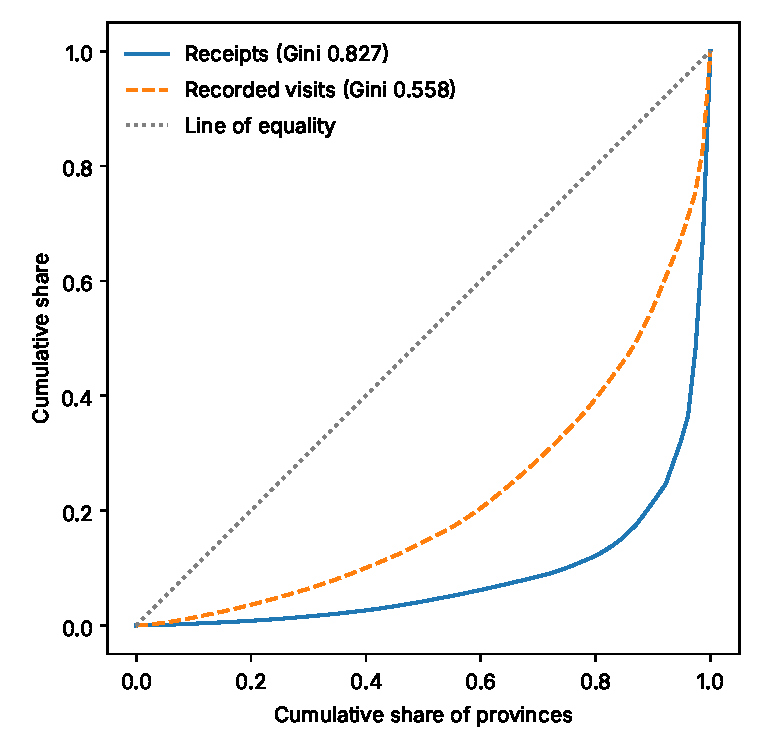
\includegraphics[width=0.62\textwidth]{results_te/fig/fig1_lorenz.pdf}
\caption{Lorenz curves of provincial tourism receipts and recorded visits, 2024. The dotted line is the line of equality. Source: author's calculations.}\label{fig:lorenz}
\end{figure}

\subsection{Between-region and within-region inequality}
The between-region component accounts for approximately 60.0\% of Theil $T$ for receipts and 54.3\% for visits. This indicates that differences among the six geographical categories account for a substantial share of the observed provincial inequality. However, inequality within regions remains important.

Bangkok is treated as a one-province geographical category. Its distinct position contributes to the between-region component. When Bangkok is excluded, the between-region share falls to 28.3\% for receipts and 17.9\% for visits (Table~\ref{tab:robust}). The decomposition should therefore be interpreted with attention to the geographical grouping and the separate treatment of Bangkok.

\subsection{Visitor composition and within-type rates}
Foreign visitors account for 23.5\% of recorded visits but 61.5\% of receipts. Average receipts per foreign recorded visit are approximately THB 21,632, compared with THB 4,162 per Thai recorded visit. The foreign-visitor yield is therefore approximately 5.2 times the Thai-visitor yield.

The accounting decomposition in Equation~(8) attributes 44.6\% of the cross-provincial variance in receipts per visit to visitor composition and 55.4\% to within-type rates. Excluding Bangkok, the composition component accounts for 44.2\% when the national benchmarks $f$, $\bar y_T$ and $\bar y_F$ are held at their 77-province values, and for 41.9\% when the benchmarks are recomputed for the 76 provinces. The Spearman rank correlation between the Punch Score and the foreign share of visits is 0.62.

Table~\ref{tab:decomp} illustrates the decomposition for selected provinces. Phuket's high yield reflects both a relatively high foreign-visitor share and high within-type receipts per visit. In Phangnga and Chiang Mai, the composition component is positive while the within-type component is negative, indicating that visitor mix alone does not explain their relative yield.

\begin{table}[t]\centering\scriptsize
\caption{Composition and within-type decomposition of receipts per visit for selected provinces, 2024}\label{tab:decomp}
\resizebox{\textwidth}{!}{\begin{tabular}{lrrrrr}
\toprule
Province & Receipts/visit (THB) & Deviation from national (THB) & Composition effect (THB) & Within-type rate effect (THB) & Foreign visits (\%) \\
\midrule
Phuket & 39,387 & 31,115 & 9,212 & 21,903 & 76.3 \\
Krabi & 16,316 & 8,045 & 5,626 & 2,419 & 55.7 \\
Bangkok & 16,023 & 7,751 & 3,939 & 3,811 & 46.1 \\
Surat Thani & 14,543 & 6,272 & 4,189 & 2,083 & 47.5 \\
Phangnga & 13,033 & 4,761 & 6,618 & $-$1,857 & 61.4 \\
Chon Buri & 12,306 & 4,034 & 3,210 & 824 & 41.9 \\
Chiang Mai & 9,312 & 1,041 & 1,287 & $-$246 & 30.9 \\
Nong Bua Lam Phu & 1,172 & $-$7,100 & $-$3,951 & $-$3,148 & 0.9 \\
\bottomrule
\end{tabular}
}\par\smallskip
\parbox{\textwidth}{\scriptsize Composition share of variance: 44.6\%; within-type rate share: 55.4\%.\\
\emph{Notes:} The composition effect is $(f_i-f)(\bar y_F-\bar y_T)$. National receipts per visit are approximately THB 4,162 for Thai visitors and THB 21,632 for foreign visitors. Variance shares are calculated as $\operatorname{Cov}(y_i,d_{k,i})/\operatorname{Var}(y_i)$ across all 77 provinces. Components may be positive or negative; the two aggregate covariance shares sum to 100\% when calculated from the same observations.}
\end{table}

\subsection{Spatial pattern}
Provincial yields exhibit positive global spatial autocorrelation under all three spatial-weight specifications (Table~\ref{tab:moran}). For the logarithm of receipts per visit, Moran's $I$ is 0.168 under inverse distance weights, 0.434 under five-nearest-neighbour weights, and 0.494 under the distance-band specification. The permutation results indicate statistical significance at the 1\% level for all statistics in the table.

The local analysis (Figure~\ref{fig:lisa}) identifies eight high-yield clusters: Krabi, Chumphon, Nakhon Si Thammarat, Phangnga, Phuket, Ranong, Surat Thani, and Trang. All are in the South. Two low-yield clusters, Mukdahan and Roi Et, are identified in the Northeast. Phatthalung is classified as a low-yield province within a high-yield neighbourhood. Khon Kaen is a borderline case: it is a high-yield province within a low-yield neighbourhood (its Punch Score of 39.7 is nevertheless below the national benchmark) with a pseudo-$p$ of 0.051 in the reported run, and it is significant in 65\% of 20 independent permutation runs, so it is not counted among the significant local patterns. The remaining 66 provinces show no statistically significant local pattern at the reported unadjusted threshold.

These local results are exploratory. Because the province-level tests are not adjusted for multiple comparisons, the number and location of significant clusters should not be interpreted as definitive evidence of local spatial processes.

\begin{table}[t]\centering\small
\caption{Global Moran's $I$ for provincial tourism indicators, 2024}\label{tab:moran}
\begin{tabular}{llrrr}
\toprule
Variable & Spatial weights & Moran's $I$ & $z$ & $p$ \\
\midrule
ln yield & Inverse distance & 0.168 & 10.82 & $<0.001$ \\
ln yield & 5 nearest neighbours & 0.434 & 7.03 & $<0.001$ \\
ln yield & Distance band & 0.494 & 5.76 & $<0.001$ \\
Punch Score & Inverse distance & 0.112 & 8.81 & $<0.001$ \\
Punch Score & 5 nearest neighbours & 0.303 & 6.04 & $<0.001$ \\
Punch Score & Distance band & 0.415 & 5.96 & $<0.001$ \\
ln receipts & Inverse distance & 0.095 & 6.36 & $<0.001$ \\
ln receipts & 5 nearest neighbours & 0.256 & 4.19 & $<0.001$ \\
ln receipts & Distance band & 0.273 & 3.23 & 0.002 \\
Foreign visitor share & Inverse distance & 0.175 & 11.06 & $<0.001$ \\
Foreign visitor share & 5 nearest neighbours & 0.373 & 6.11 & $<0.001$ \\
Foreign visitor share & Distance band & 0.537 & 6.25 & $<0.001$ \\
\bottomrule
\end{tabular}
\par\smallskip
\parbox{0.9\textwidth}{\scriptsize\emph{Notes:} All weights are row-standardised and based on great-circle distances between province centroids. The specifications are inverse distance, five nearest neighbours, and a distance band (the smallest distance at which every province has a neighbour, 111.6 km). Inference uses 9,999 random permutations. The null expectation of Moran's $I$ is $-1/76=-0.0132$ for 77 observations.}
\end{table}

\begin{figure}[t]\centering
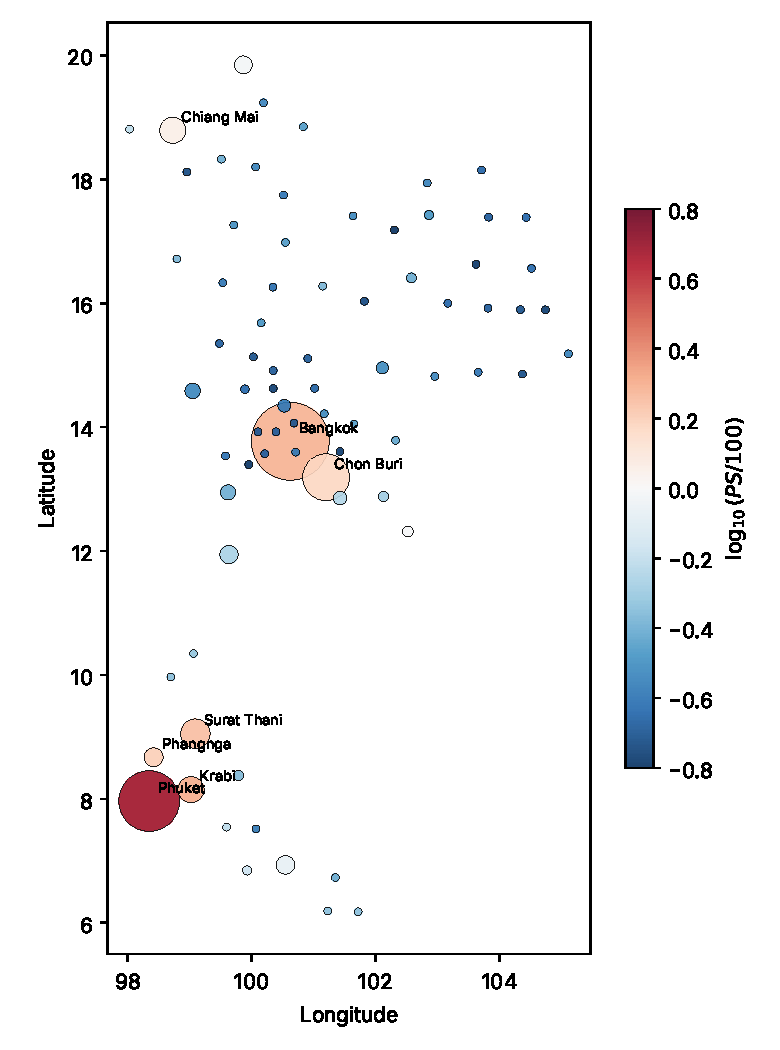
\includegraphics[width=0.62\textwidth]{results_te/fig/fig2_yield_map.pdf}
\caption{Provincial centroids and tourism yield, 2024. Bubble area is proportional to tourism receipts (a minimum marker size is applied for visibility). Colour shows $\log_{10}(\PS/100)$ on a diverging scale centred on the national average ($\PS=100$). Source: author's calculations.}\label{fig:map}
\end{figure}
\begin{figure}[t]\centering
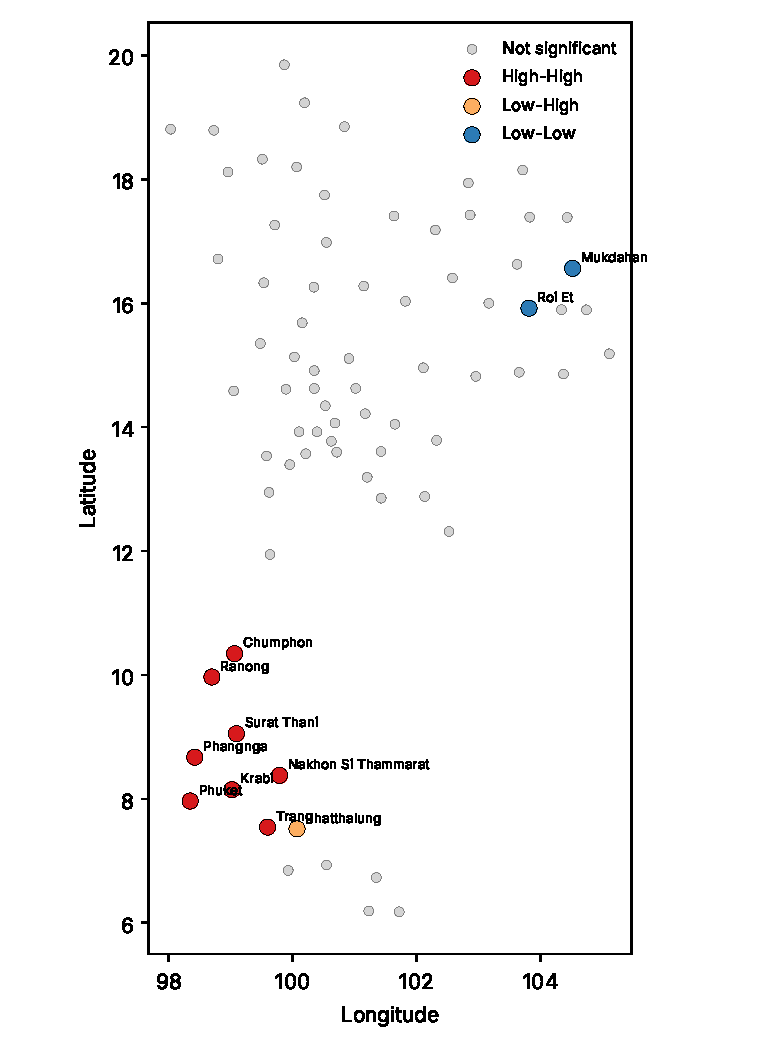
\includegraphics[width=0.62\textwidth]{results_te/fig/fig3_lisa.pdf}
\caption{Local indicators of spatial association (LISA) for provincial tourism yield (logarithm of receipts per visit) in Thailand, 2024, computed at provincial centroids. High--High and Low--Low clusters indicate positive local spatial association, while High--Low and Low--High indicate spatial outliers. Source: author's calculations.}\label{fig:lisa}
\end{figure}

\subsection{Correlates of yield and tourism intensity}
Table~\ref{tab:corr} reports Spearman rank correlations between the Punch Score and selected provincial variables. The Punch Score is positively associated with the foreign share of visits, length of stay, occupancy, the ratio of accommodation guests to recorded visits, and rooms per 1,000 visits. Its association with GPP per capita is positive but comparatively weak.

The correlation with average daily expenditure is particularly high ($\rho=0.97$). This should not be interpreted as independent evidence that expenditure explains yield, because the expenditure and receipts variables originate from the same tourism-statistics system and may share underlying measurement components. The same caution applies, to a lesser degree, to length of stay.

Tourism receipts are equivalent to 15.7\% of national GPP at current prices and approximately 14.8\% in Bangkok. The corresponding ratios are approximately 210\% in Phuket and 111\% in Krabi. These ratios compare gross tourism receipts with GPP and should be interpreted as indicators of tourism intensity rather than tourism's contribution to provincial value added. Gross receipts and GPP are conceptually different measures and should not be treated as directly interchangeable.

\begin{table}[t]\centering\small
\caption{Spearman rank correlations with the Punch Score, 2024}\label{tab:corr}
\resizebox{\textwidth}{!}{\begin{tabular}{lrrrr}
\toprule
Variable & $\rho$ (77) & $p$ & $\rho$ (excluding Bangkok) & $p$ \\
\midrule
Foreign visitor share (\%) & 0.62 & $<0.001$ & 0.61 & $<0.001$ \\
Average daily expenditure (THB/person/day)$^\dagger$ & 0.97 & $<0.001$ & 0.97 & $<0.001$ \\
Average length of stay (days)$^\dagger$ & 0.72 & $<0.001$ & 0.71 & $<0.001$ \\
Occupancy rate (\%) & 0.60 & $<0.001$ & 0.59 & $<0.001$ \\
Accommodation guests / visitors (\%) & 0.77 & $<0.001$ & 0.77 & $<0.001$ \\
Rooms per 1,000 visits & 0.73 & $<0.001$ & 0.73 & $<0.001$ \\
GPP per capita (THB) & 0.27 & 0.018 & 0.24 & 0.036 \\
Visitors per resident & 0.41 & $<0.001$ & 0.39 & $<0.001$ \\
\bottomrule
\end{tabular}
}\par\smallskip
\parbox{\textwidth}{\scriptsize\emph{Notes:} These are descriptive rank correlations, not causal estimates. $\dagger$ Expenditure and length of stay come from the same tourism-statistics system as receipts, so their correlations with receipts per visit are partly definitional and are not independent evidence. Rooms per 1,000 visits and GPP per capita are computed from the assembled provincial variables.}
\end{table}

\subsection{Robustness}\label{sec:robust}
Table~\ref{tab:robust} compares the baseline results with a specification that excludes Bangkok. Excluding Bangkok, the Gini coefficients remain high at 0.773 for receipts and 0.492 for visits. When the Punch Score is re-benchmarked to the 76-province average, nine provinces exceed 100.

\begin{table}[t]\centering\small
\caption{Robustness of the main results, 2024}\label{tab:robust}
\resizebox{\textwidth}{!}{\begin{tabular}{lrr}
\toprule
Statistic & Baseline (77 provinces) & Excluding Bangkok (76 provinces) \\
\midrule
Total receipts (M THB) & 2,924,506.59 & 1,982,313.45 \\
Total visits & 353,556,836 & 294,752,564 \\
Gini, receipts & 0.827 & 0.773 \\
Gini, visits & 0.558 & 0.492 \\
Theil $T$, receipts & 1.765 & 1.454 \\
Theil $T$, visits & 0.639 & 0.427 \\
Between-region share, receipts (\%) & 60.0 & 28.3 \\
Between-region share, visits (\%) & 54.3 & 17.9 \\
Provinces with Punch Score $>100$ & 7 & 9 \\
Median Punch Score & 29.2 & 35.7 \\
\bottomrule
\end{tabular}
}\par\smallskip
\parbox{\textwidth}{\scriptsize\emph{Notes:} Baseline results use the revised Ministry of Tourism and Sports workbook identified as revised on 28 August 2025. The Bangkok-excluded specification uses 76 provinces, recomputes the five regional groups, and re-benchmarks the Punch Score to the 76-province average.}
\end{table}

\section{Discussion and limitations}
The principal finding is that tourism receipts are more geographically concentrated than recorded visits. A relatively small number of provinces account for a large share of receipts, while many provinces record substantial visit volumes but relatively low receipts per visit. The difference is associated with both visitor composition and within-type receipts per visit. This pattern is consistent with the established literature on heterogeneity in tourist expenditure \citep{wang2010,brida2013} and with broader accounts of geographical concentration in economic activity \citep{krugman1991}. However, the present data cannot identify the mechanisms that generate these patterns.

The visitor-composition decomposition indicates that approximately 44.6\% of cross-provincial variance in receipts per visit is associated with differences in the foreign-visitor share. The remaining 55.4\% is associated with within-type receipts per visit. This distinction matters for interpretation: a province may have a high yield because it receives a larger proportion of foreign visitors, because visitors of a given type spend more per visit, or because both conditions occur. The decomposition is an accounting identity and should not be interpreted as a causal attribution.

The spatial results indicate positive spatial association, particularly among southern provinces. This pattern is compatible with shared destination markets, transport connectivity, tourism corridors, or other regional characteristics. Nevertheless, spatial autocorrelation does not demonstrate that one province's tourism performance causes a neighbouring province's performance to change. The results are based on centroid-distance weights and do not directly model interprovincial economic interactions.

For tourism monitoring, the findings suggest that visitor volumes and receipts per visit should be reported together. Regional comparisons should also distinguish Thai and foreign visitors. A high Punch Score should not automatically be interpreted as a reason to allocate more public support, and a low score should not be interpreted as evidence of poor destination management. Provinces with lower receipts per visit may serve domestic mobility, cultural, family, or regional travel functions that are not captured by gross tourism receipts.

Several limitations should be considered. First, the analysis covers only 2024. The observed distribution may reflect post-pandemic recovery, temporary demand conditions, or other year-specific factors. A multi-year provincial panel would be necessary to assess whether the observed patterns are persistent.

Second, recorded visits are not unique travellers. A person visiting multiple provinces may be counted in more than one provincial total. The resulting measure is appropriate for describing recorded destination activity, but it should not be interpreted as the number of distinct travellers or national trips.

Third, receipts are nominal gross estimates and are not adjusted for provincial price differences. They do not measure local value added, household income, or the proportion of spending retained within the destination economy. Differences in local prices, business ownership, supply-chain leakages, and the structure of tourism services may affect the relationship between gross receipts and local economic benefits.

Fourth, the Punch Score used here is a rescaled measure of receipts per recorded visit. It is the single-criterion, risk-neutral special case of the Punch Score framework described in Section~\ref{sec:ps}, not the weighted multi-criteria framework, and it is not a measure of productivity, technical efficiency, destination competitiveness, or welfare. Its purpose is to make the relative-yield dimension explicit alongside the volume of recorded visits.

Fifth, provinces are equally weighted in the baseline inequality measures. This treats each province as one geographical unit, regardless of population or economic size. The population-weighted sensitivity analysis provides an alternative perspective, but it does not replace the baseline provincial comparison.

Sixth, the spatial analysis uses distances between province centroids rather than shared boundaries. Centroid-based weights provide a consistent distance measure but may not represent actual transport connectivity, travel time, or geographical interaction. Local Moran results are also exploratory because the reported local significance threshold is not adjusted for multiple testing, and the classification of provinces near the threshold (Khon Kaen) is not stable across permutation seeds.

Finally, the study is descriptive and does not include provincial public expenditure, tourism investment, or detailed input--output information. It cannot determine whether public spending raises tourism yield or whether high gross receipts translate into greater local economic benefits. Future work could combine multi-year provincial data with provincial price indices, input--output tables, fiscal expenditure, and more detailed visitor microdata to investigate these questions.

\section{Conclusion}
Across Thailand's 77 provinces in 2024, tourism receipts are more concentrated than recorded visits. The Gini coefficients are 0.827 for receipts and 0.558 for visits. Bangkok and the South together account for 65.9\% of receipts and 33.2\% of recorded visits. Seven provinces exceed the national relative-yield benchmark, and foreign visitors account for a substantially larger share of receipts than of visits.

The visitor-composition decomposition indicates that approximately 44.6\% of cross-provincial variance in receipts per visit is associated with differences in the foreign-visitor share, while the remainder is associated with within-type receipts per visit. Positive spatial autocorrelation is also observed, with high-yield clustering concentrated in southern provinces. The principal concentration findings remain high when Bangkok is excluded, although the between-region share of inequality falls substantially.

The Punch Score is a transparent relative-yield indicator. Its value lies in distinguishing the volume of recorded visits from the receipts associated with those visits. It should be interpreted alongside visitor composition, distributional measures, and spatial analysis rather than as a stand-alone ranking of provincial tourism performance.

The provincial assessment provides a descriptive baseline for future multi-year research on tourism receipts, regional development, and the geographical distribution of tourism-generated economic activity.

\section*{Data and code availability}
The 77-province dataset constructed from the cited public sources, the scripts that build and validate it, the analysis code that produces every table and figure, and a script that checks every quoted number against the recomputation are reproduced in the supplementary material and archived at Zenodo (\url{https://doi.org/\RepoDOI}), together with the random seeds. \todo{Replace the identifier in \texttt{\textbackslash RepoDOI} (top of this file and of \texttt{title\_page.tex}) by the DOI of the Zenodo release that contains the corrected files; the DOI of any earlier, incorrect upload must not be used.}

\bibliographystyle{plainnat}
\begin{thebibliography}{99}\small
\bibitem[Alam and Paramati(2016)]{alam2016} Alam MS and Paramati SR (2016) The impact of tourism on income inequality in developing economies: Does Kuznets curve hypothesis exist? \emph{Annals of Tourism Research} 61: 111--126. \url{https://doi.org/10.1016/j.annals.2016.09.008}.
\bibitem[Anonymous(2026a)]{anon2026} Anonymous (2026a) Methodological work on feedback-driven estimation of Punch Score weights. Manuscript under review; details omitted for anonymous review.
\bibitem[Anonymous(2026b)]{anon2026b} Anonymous (2026b) A conceptual weighted Punch Score framework for research assessment. Manuscript under review or in production; details omitted for anonymous review.
\bibitem[Anselin(1995)]{anselin1995} Anselin L (1995) Local indicators of spatial association---LISA. \emph{Geographical Analysis} 27(2): 93--115. \url{https://doi.org/10.1111/j.1538-4632.1995.tb00338.x}.
\bibitem[Balaguer and Cantavella-Jord\'a(2002)]{balaguer2002} Balaguer J and Cantavella-Jord\'a M (2002) Tourism as a long-run economic growth factor: The Spanish case. \emph{Applied Economics} 34(7): 877--884.
\bibitem[Balassa(1965)]{balassa1965} Balassa B (1965) Trade liberalisation and ``revealed'' comparative advantage. \emph{The Manchester School} 33(2): 99--123.
\bibitem[Brida and Scuderi(2013)]{brida2013} Brida JG and Scuderi R (2013) Determinants of tourist expenditure: A review of microeconometric models. \emph{Tourism Management Perspectives} 6: 28--40. \url{https://doi.org/10.1016/j.tmp.2012.10.006}.
\bibitem[Brida et~al.(2016)]{brida2016} Brida JG, Cortes-Jimenez I and Pulina M (2016) Has the tourism-led growth hypothesis been validated? A literature review. \emph{Current Issues in Tourism} 19(5): 394--430. \url{https://doi.org/10.1080/13683500.2013.868414}.
\bibitem[Cowell(2011)]{cowell2011} Cowell FA (2011) \emph{Measuring Inequality}, 3rd edn. Oxford: Oxford University Press.
\bibitem[Dwyer and Kim(2003)]{dwyer2003} Dwyer L and Kim C (2003) Destination competitiveness: Determinants and indicators. \emph{Current Issues in Tourism} 6(5): 369--414.
\bibitem[Isard(1960)]{isard1960} Isard W (1960) \emph{Methods of Regional Analysis: An Introduction to Regional Science}. Cambridge, MA: MIT Press.
\bibitem[Krugman(1991)]{krugman1991} Krugman P (1991) Increasing returns and economic geography. \emph{Journal of Political Economy} 99(3): 483--499.
\bibitem[Ministry of Tourism and Sports(2025a)]{mots2025a} Ministry of Tourism and Sports (2025a) \emph{Provincial Tourism Statistics, January--December 2024: Revised 28 August 2025; and Domestic Tourism Statistics, Q1--Q4 2024}. Bangkok: Ministry of Tourism and Sports. \url{https://secretary.mots.go.th/tourism-stat} (accessed 10 November 2026).
\bibitem[Moran(1950)]{moran1950} Moran PAP (1950) Notes on continuous stochastic phenomena. \emph{Biometrika} 37(1--2): 17--23. \url{https://doi.org/10.1093/biomet/37.1-2.17}.
\bibitem[National Economic and Social Development Council(2025)]{nesdc2025} National Economic and Social Development Council (2025) \emph{Gross Regional and Provincial Product 2024: Excel Tables}. Bangkok: NESDC. \url{https://www.nesdc.go.th/en/download/table-of-gross-regional-and-provincial-product-2024-excel/} (accessed 10 November 2026).
\bibitem[National Statistical Office(2025)]{nso2025} National Statistical Office (2025) \emph{Statistical Yearbook Thailand 2025}. Bangkok: National Statistical Office. Table 1.5, registered population by province.
\bibitem[National Statistical Office(2026)]{nso2026} National Statistical Office (2026) \emph{Statistical Yearbook Thailand 2026}. Bangkok: National Statistical Office. \url{https://www.nso.go.th/public/e-book/Statistical-Yearbook/SYB-2026_webPage/Page_SYB_EN.html} (accessed 10 November 2026).
\bibitem[OCHA(2019)]{ocha2019} United Nations Office for the Coordination of Humanitarian Affairs [OCHA] (2019) Thailand Subnational Administrative Boundaries (COD-AB): tha\_admbnda\_adm1\_rtsd\_20190221. Humanitarian Data Exchange. \url{https://data.humdata.org} (accessed 10 November 2026).
\bibitem[Shorrocks(1980)]{shorrocks1980} Shorrocks AF (1980) The class of additively decomposable inequality measures. \emph{Econometrica} 48(3): 613--625. \url{https://doi.org/10.2307/1913126}.
\bibitem[Theil(1967)]{theil1967} Theil H (1967) \emph{Economics and Information Theory}. Amsterdam: North-Holland.
\bibitem[Wang and Davidson(2010)]{wang2010} Wang Y and Davidson MCG (2010) A review of micro-analyses of tourist expenditure. \emph{Current Issues in Tourism} 13(6): 507--524. \url{https://doi.org/10.1080/13683500903406359}.
\bibitem[Williamson(1965)]{williamson1965} Williamson JG (1965) Regional inequality and the process of national development: A description of the patterns. \emph{Economic Development and Cultural Change} 13(4, Part 2): 1--84.
\end{thebibliography}

\appendix
\section{Provincial Punch Scores and components}
The provincial Punch Score is the dimensionless relative-yield index defined in Section~\ref{sec:ps}. It is normalized to a national benchmark of 100 and is not a percentage. Values above 100 indicate receipts per recorded visit above the national average; values below 100 indicate receipts per recorded visit below the national average. Provinces are ranked by unrounded scores.
\begin{center}\scriptsize
\captionof{table}{Punch Score and tourism components for all 77 provinces, 2024}\label{tab:all}
\begin{longtable}{rllrrrrr}
\toprule
Rank & Province & Region & Visits & Receipts (M THB) & Receipts/visit (THB) & Punch Score (index) & Foreign visits (\%) \\
\midrule
\endfirsthead
\toprule
Rank & Province & Region & Visits & Receipts (M THB) & Receipts/visit (THB) & Punch Score (index) & Foreign visits (\%) \\
\midrule
\endhead
\bottomrule
\endfoot
1 & Phuket & South & 14,511,188 & 571,550.00 & 39,387 & 476.2 & 76.3 \\
2 & Krabi & South & 6,470,693 & 105,578.45 & 16,316 & 197.3 & 55.7 \\
3 & Bangkok & Bangkok & 58,804,272 & 942,193.14 & 16,023 & 193.7 & 46.1 \\
4 & Surat Thani & South & 9,198,788 & 133,781.02 & 14,543 & 175.8 & 47.5 \\
5 & Phangnga & South & 4,258,670 & 55,501.97 & 13,033 & 157.6 & 61.4 \\
6 & Chon Buri & East & 27,898,229 & 343,303.14 & 12,306 & 148.8 & 41.9 \\
7 & Chiang Mai & North & 11,473,206 & 106,844.16 & 9,312 & 112.6 & 30.9 \\
8 & Trat & East & 2,235,315 & 18,138.30 & 8,114 & 98.1 & 18.7 \\
9 & Chiang Rai & North & 6,282,437 & 49,438.70 & 7,869 & 95.1 & 13.1 \\
10 & Songkhla & South & 7,437,817 & 53,175.22 & 7,149 & 86.4 & 54.9 \\
11 & Satun & South & 2,342,623 & 13,084.86 & 5,586 & 67.5 & 19.7 \\
12 & Mae Hong Son & North & 1,326,887 & 6,771.41 & 5,103 & 61.7 & 19.2 \\
13 & Trang & South & 1,729,099 & 8,682.44 & 5,021 & 60.7 & 5.2 \\
14 & Rayong & East & 6,102,399 & 28,859.16 & 4,729 & 57.2 & 16.8 \\
15 & Prachuap Khiri Khan & Central & 11,313,134 & 51,697.81 & 4,570 & 55.2 & 6.7 \\
16 & Chanthaburi & East & 3,736,074 & 15,992.58 & 4,281 & 51.7 & 0.9 \\
17 & Chumphon & South & 1,839,178 & 7,208.52 & 3,919 & 47.4 & 2.7 \\
18 & Yala & South & 1,963,459 & 7,392.08 & 3,765 & 45.5 & 43.8 \\
19 & Ranong & South & 925,281 & 3,483.21 & 3,764 & 45.5 & 3.5 \\
20 & Narathiwat & South & 1,191,069 & 4,469.55 & 3,753 & 45.4 & 59.2 \\
21 & Nakhon Si Thammarat & South & 4,336,613 & 15,726.83 & 3,627 & 43.8 & 1.4 \\
22 & Phetchabun & North & 2,701,223 & 9,500.57 & 3,517 & 42.5 & 2.1 \\
23 & Tak & North & 2,252,535 & 7,858.74 & 3,489 & 42.2 & 2.2 \\
24 & Phetchaburi & Central & 10,695,183 & 35,728.03 & 3,341 & 40.4 & 2.6 \\
25 & Khon Kaen & Northeast & 4,682,491 & 15,376.46 & 3,284 & 39.7 & 2.6 \\
26 & Lampang & North & 1,757,258 & 5,725.86 & 3,258 & 39.4 & 6.1 \\
27 & Pattani & South & 618,737 & 1,988.34 & 3,214 & 38.9 & 28.2 \\
28 & Sa Kaeo & East & 1,597,969 & 5,015.43 & 3,139 & 37.9 & 7.8 \\
29 & Prachin Buri & East & 1,488,044 & 4,340.47 & 2,917 & 35.3 & 1.6 \\
30 & Phitsanulok & North & 3,141,098 & 9,079.45 & 2,891 & 34.9 & 5.8 \\
31 & Nan & North & 1,558,649 & 4,503.88 & 2,890 & 34.9 & 1.7 \\
32 & Udon Thani & Northeast & 4,951,386 & 13,601.12 & 2,747 & 33.2 & 21.4 \\
33 & Nakhon Sawan & North & 2,347,611 & 6,386.12 & 2,720 & 32.9 & 0.8 \\
34 & Sukhothai & North & 1,370,515 & 3,545.47 & 2,587 & 31.3 & 22.4 \\
35 & Nakhon Ratchasima & Northeast & 8,886,543 & 22,715.42 & 2,556 & 30.9 & 2.7 \\
36 & Nakhon Nayok & East & 2,968,262 & 7,335.65 & 2,471 & 29.9 & 0.6 \\
37 & Loei & Northeast & 2,273,467 & 5,565.46 & 2,448 & 29.6 & 1.5 \\
38 & Kanchanaburi & Central & 15,006,038 & 36,563.95 & 2,437 & 29.5 & 2.8 \\
39 & Buri Ram & Northeast & 3,892,049 & 9,403.66 & 2,416 & 29.2 & 1.6 \\
40 & Phayao & North & 1,037,898 & 2,478.72 & 2,388 & 28.9 & 4.2 \\
41 & Ubon Ratchathani & Northeast & 3,808,230 & 8,996.66 & 2,362 & 28.6 & 1.1 \\
42 & Phrae & North & 1,322,332 & 3,118.96 & 2,359 & 28.5 & 1.9 \\
43 & Nong Khai & Northeast & 3,667,972 & 8,614.85 & 2,349 & 28.4 & 31.3 \\
44 & Phra Nakhon Si Ayutthaya & Central & 11,333,205 & 24,940.34 & 2,201 & 26.6 & 17.6 \\
45 & Phatthalung & South & 1,845,345 & 4,045.13 & 2,192 & 26.5 & 4.6 \\
46 & Samut Prakan & Central & 4,141,005 & 8,926.85 & 2,156 & 26.1 & 24.9 \\
47 & Kamphaeng Phet & North & 873,706 & 1,859.15 & 2,128 & 25.7 & 3.3 \\
48 & Uttaradit & North & 1,110,726 & 2,327.74 & 2,096 & 25.3 & 0.7 \\
49 & Surin & Northeast & 1,271,977 & 2,657.93 & 2,090 & 25.3 & 2.7 \\
50 & Ratchaburi & Central & 3,089,469 & 6,279.79 & 2,033 & 24.6 & 4.4 \\
51 & Phichit & North & 831,127 & 1,638.56 & 1,971 & 23.8 & 0.3 \\
52 & Mukdahan & Northeast & 1,863,075 & 3,577.02 & 1,920 & 23.2 & 7.7 \\
53 & Suphan Buri & Central & 5,738,470 & 10,892.65 & 1,898 & 22.9 & 0.9 \\
54 & Maha Sarakham & Northeast & 661,375 & 1,237.98 & 1,872 & 22.6 & 1.7 \\
55 & Nakhon Phanom & Northeast & 2,262,163 & 4,224.67 & 1,868 & 22.6 & 7.6 \\
56 & Bueng Kan & Northeast & 929,701 & 1,715.88 & 1,846 & 22.3 & 3.7 \\
57 & Saraburi & Central & 4,857,377 & 8,810.16 & 1,814 & 21.9 & 1.7 \\
58 & Uthai Thani & North & 1,026,793 & 1,808.88 & 1,762 & 21.3 & 0.2 \\
59 & Samut Sakhon & Central & 1,559,280 & 2,739.53 & 1,757 & 21.2 & 0.9 \\
60 & Sakon Nakhon & Northeast & 1,854,233 & 3,237.73 & 1,746 & 21.1 & 1.1 \\
61 & Roi Et & Northeast & 934,719 & 1,621.48 & 1,735 & 21.0 & 1.6 \\
62 & Nonthaburi & Central & 4,106,144 & 7,122.12 & 1,735 & 21.0 & 6.0 \\
63 & Sing Buri & Central & 920,395 & 1,576.52 & 1,713 & 20.7 & 0.8 \\
64 & Lop Buri & Central & 4,460,768 & 7,635.92 & 1,712 & 20.7 & 0.7 \\
65 & Nakhon Pathom & Central & 4,698,158 & 7,784.35 & 1,657 & 20.0 & 1.7 \\
66 & Pathum Thani & Central & 3,451,311 & 5,651.75 & 1,638 & 19.8 & 11.2 \\
67 & Chai Nat & Central & 1,214,902 & 1,966.99 & 1,619 & 19.6 & 0.6 \\
68 & Yasothon & Northeast & 625,815 & 1,004.50 & 1,605 & 19.4 & 0.6 \\
69 & Si Sa Ket & Northeast & 1,158,400 & 1,818.04 & 1,569 & 19.0 & 0.6 \\
70 & Lamphun & North & 1,334,200 & 2,049.49 & 1,536 & 18.6 & 5.7 \\
71 & Chaiyaphum & Northeast & 1,988,320 & 3,042.51 & 1,530 & 18.5 & 0.5 \\
72 & Amnat Charoen & Northeast & 287,173 & 408.18 & 1,421 & 17.2 & 2.3 \\
73 & Ang Thong & Central & 1,173,127 & 1,660.12 & 1,415 & 17.1 & 1.0 \\
74 & Chachoengsao & East & 6,172,758 & 8,678.41 & 1,406 & 17.0 & 0.7 \\
75 & Kalasin & Northeast & 2,401,692 & 3,264.38 & 1,359 & 16.4 & 1.7 \\
76 & Samut Songkhram & Central & 5,610,458 & 7,555.23 & 1,347 & 16.3 & 2.9 \\
77 & Nong Bua Lam Phu & Northeast & 367,548 & 430.79 & 1,172 & 14.2 & 0.9 \\
\end{longtable}

\end{center}
{\scriptsize\emph{Notes:} Revised Ministry of Tourism and Sports workbook, identified as revised on 28 August 2025. The Punch Score is a dimensionless relative-yield index normalized to 100; it is not a percentage. Provinces are ranked by unrounded Punch Score.}

\section{Local clusters and stability of the classification}
\begin{table}[h]\centering\small
\caption{Significant local Moran statistics for the logarithm of receipts per visit (five nearest neighbours, 9,999 conditional permutations, two-sided pseudo-$p<0.05$, unadjusted) and provinces significant in at least 25\% of 20 independent permutation runs}\label{tab:lisa}
\begin{tabular}{llcrrr}
\toprule
Province & Region & Cluster type & Local $I_i$ & Pseudo-$p$ & Significant in (\% of 20 seeds) \\
\midrule
Krabi & South & High-High & 4.72 & $<0.001$ & 100 \\
Chumphon & South & High-High & 0.50 & 0.010 & 100 \\
Nakhon Si Thammarat & South & High-High & 0.46 & 0.002 & 100 \\
Phangnga & South & High-High & 4.06 & $<0.001$ & 100 \\
Phuket & South & High-High & 6.17 & $<0.001$ & 100 \\
Ranong & South & High-High & 0.57 & 0.002 & 100 \\
Surat Thani & South & High-High & 2.71 & 0.009 & 100 \\
Trang & South & High-High & 0.73 & 0.028 & 100 \\
Phatthalung & South & Low-High & $-$0.49 & 0.013 & 100 \\
Mukdahan & Northeast & Low-Low & 0.55 & 0.038 & 100 \\
Roi Et & Northeast & Low-Low & 0.66 & 0.044 & 100 \\
Khon Kaen & Northeast & High-Low & $-$0.14 & 0.051 & 65 \\
\bottomrule
\end{tabular}

\end{table}
\end{document}
